\section{Introduction}

\begin{frame}{Motivation}
\begin{itemize}
    \item Graph machine learning can be tracked backwards to the problem of `learning' on data that is inherently a graph \cite{silva2016machine, JMLR:Perozzi} or can be modeled as a graph \cite{verri2013,grape2020}
    \item Variety of tasks:  node/edge classification, link prediction, graph partitioning, which rely on learning representations from graph-structured data.
    \item  Techniques were most developed by complex networks researchers.
    \item \textbf{Last decade:} significant shift towards the merging of three main communities: graph signal processing, deep learning and complex nets.

\end{itemize}
\end{frame}


\begin{frame}{GraphML paradigms Overview}
    \begin{itemize}
        \item Three main learning paradigms: supervised, unsupervised, and semi-supervised learning
        \item We are interested on the (semi-)supervised learning paradigm, which encompasses a variety of techniques designed to leverage learning to (partially-)labeled data \cite{verri2018advantages,amanciof}
        \item  Focus in the subset of graph elements (nodes,edges,graph structure) prediction(classification/regression) methods.
        \item Consider the division of the field into \texttt{traditional} graph learning: topological graph measures into `tabular' ML algorithms  \cite{costa2007characterization, silva2016machine}, and \texttt{deep} graph learning
    \end{itemize}
\end{frame}

\begin{frame}{Brief History}
    \begin{itemize}
        \item The beggining of the field was focused in Complex Networks (CNet) techniques \cite{costa2007characterization, silva2016machine}
        \item Graph Signal Processing (GSP) techniques were used in the first spectral graph neural network (GNN) \cite{bruna2013spectral}
        \item In the mean time, the CNet community was developing the first deep node embedding techiniques : DeepWalk \cite{perozzi2014deepwalk} and node2vec \cite{grover2016node2vec}
        \item The advent of new GNN architectures, such as Graph Convolutional Network (GCN) \cite{kipf2016semi} and GraphSAGE \cite{hamilton2017inductive}, represented a unification of the field.
    \end{itemize}
\end{frame}

\begin{frame}{Traditional Graph Learning}
    \begin{itemize}
        \item Early efforts were focused on developing graph-based features that could be integrated in standard ML algorithms: logistic regression, decision trees, SVM.
        \item Among these features, centrality measures became important: capturing the influence of `nodes' \cite{bonacich1987power} in the network.
        \item However, centrality measures can also capture information of higher-order structures, such as edges \cite{Lu2013edgebetw} and hyperedges \cite{tudisco2021hyperedge}.
        \item This adaptative power of centrality possibilitate GraphML in different tasks, such as node classification, link prediction, and hyperedge feature prediction.
    \end{itemize}
\end{frame}

\begin{frame}{Deep Graph Learning}
    \begin{itemize}
        \item Revolutionized the field of Graph ML, where GNNs are now end-to-end trainable models responsible for the tasks described earlier.
        \item GNNs can be divided into two main categories: spectral-based and spatial-based.
        \item A common mistake is to classify GCN as spatial-based, when it is in fact a spectral method that can be understood as a spatial message passing.
        \item In this presentation, we will focus on differentiate spatial and spectral, focusing on  Graph Attention Networks (GATs) vs spectral architectures.
    \end{itemize}
\end{frame}


% \begin{frame}{Traditional graph learning}
%     \begin{figure}
%       \begin{columns}
%         \column{.3\linewidth}
%         \caption{Drones Congestion in a high-traffic Last Mile Delivery context. \\ Source: \cite{imageDronesCongestion}}
%         \label{fig:example left}
%         \column{.65\linewidth}
%         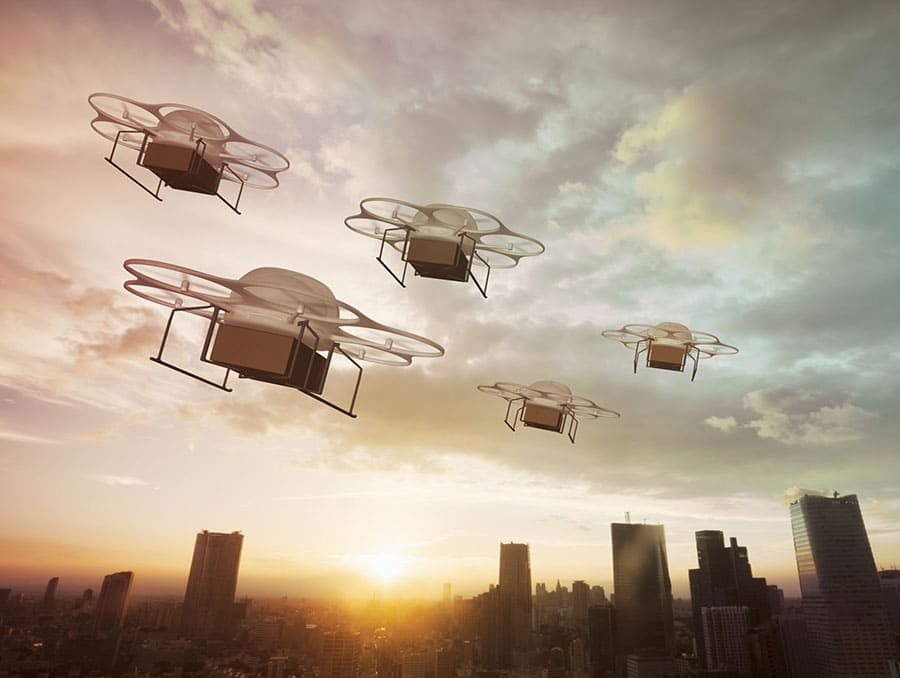
\includegraphics[width=\textwidth]{img/Drone Congestion.jpg}
%       \end{columns}
%     \end{figure}

% \end{frame}

% \begin{frame}{Introduction to Last-Mile Delivery Drones}
% \destaq{Last Mile Delivery Drones (LMDD)}
% \begin{itemize}
%     \item Heterogeneous research area:
%     \begin{itemize}
%         \item Combining drones and trucks.
%         \item Linear integer modeling.
%         \item Fuzzy logic for uncertainties.
%         \item Multi-objective optimization.
%         \item Exclusive drone-based solutions.
%     \end{itemize}
%     \item \textbf{Complex Systems Decentralized Approach}:
%     \begin{itemize}
%         \item Tradable permit model for multi-agent airspace use \cite{Verri}.
%     \end{itemize}
% \end{itemize}

% \end{frame}

% \begin{frame}{Related Work and Centralized Control}
% \begin{itemize}
%     \item \textbf{Necessity of Air Traffic Management}:
%     \begin{itemize}
%         \item Most centralized models don't address collision avoidance \cite{DUKKANCI2023}.
%         \item Ensuring optimal path planning and efficient airspace control.
%     \end{itemize}
%     \item \textbf{Centralized Control and UTM}:
%     \begin{itemize}
%         \item \textbf{Centralized Control}:
%         \begin{itemize}
%             \item Federal Aviation Administration (FAA) and NASA's Unmanned Aircraft System Traffic Management (UTM) \cite{nasa}.
%             \item Ensures organized, legislative-backed airspace control.
%         \end{itemize}
%         \item \textbf{Decentralized Models}:
%         \begin{itemize}
%             \item Novel but complex in scalability and regulatory compliance.
%         \end{itemize}
%     \end{itemize}
% \end{itemize}
% \end{frame}


% \begin{frame}{Proposed Approach}
% \begin{itemize}
%     \item \textbf{Aispace Control and MAPF Approach}:
%     \begin{itemize}
%         \item Multi-Agent Path Finding (MAPF) is a solution for addressing spatial characteristics and collision avoidance.
%     \end{itemize}
%     \item \textbf{Proposed Strategy}:
%     \begin{itemize}
%         \item Employing MAPF strategy for Last Mile Delivery Drone problem.
%         \item Three approaches: MILP, heuristic and hybrid.
%         \item Use of prioritized planning \cite{7138650} and conflict-based search \cite{SHARON201540} to manage computational complexity in the heuristic.
%         \item Comparing the MILP with the heuristic.
%         \item Qualitative comparison between centralized and decentralized approaches.
%     \end{itemize}
% \end{itemize}
% \end{frame}
